\documentclass[a4paper,12pt]{article}
\usepackage{titling}
\usepackage{lscape}
\usepackage{amssymb, amsmath, amssymb}
\usepackage{booktabs}
\usepackage{makecell}
\usepackage{float}
\floatplacement{figure}{H}
\usepackage[stable]{footmisc}
\usepackage{lmodern}
\usepackage{microtype}
\usepackage{libertine}
\usepackage[libertine]{newtxmath}
\usepackage[scale=.8]{FiraMono}
\usepackage[usenames, dvipsnames]{xcolor}
\usepackage{setspace}
\usepackage{float}
\usepackage[top=2cm, bottom=2cm, left=2cm, right=2cm]{geometry}
\usepackage{graphicx}
\usepackage{xcolor}
\definecolor{darkblue}{rgb}{0.0,0.0,0.55}
\usepackage{dcolumn}
\usepackage{mathtools}
\usepackage{caption}
\usepackage[UKenglish]{babel}
\usepackage[UKenglish]{isodate}
\usepackage[authoryear]{natbib}
\usepackage{babelbib}
\usepackage{bibentry}
\cleanlookdateon
\exhyphenpenalty=10000
\hyphenpenalty=10000
\widowpenalty=10000
\clubpenalty=10000
\setcitestyle{aysep={}} 
\usepackage{etoolbox}
\makeatletter
\patchcmd{\NAT@citex}
	  {\@citea\NAT@hyper@{%
		 \NAT@nmfmt{\NAT@nm}%
		 \hyper@natlinkbreak{\NAT@aysep\NAT@spacechar}{\@citeb\@extra@b@citeb}%
		 \NAT@date}}
	  {\@citea\NAT@nmfmt{\NAT@nm}%
	   \NAT@aysep\NAT@spacechar\NAT@hyper@{\NAT@date}}{}{}
	\patchcmd{\NAT@citex}
	  {\@citea\NAT@hyper@{%
		 \NAT@nmfmt{\NAT@nm}%
		 \hyper@natlinkbreak{\NAT@spacechar\NAT@@open\if*#1*\else#1\NAT@spacechar\fi}%
		   {\@citeb\@extra@b@citeb}%
		 \NAT@date}}
	  {\@citea\NAT@nmfmt{\NAT@nm}%
	   \NAT@spacechar\NAT@@open\if*#1*\else#1\NAT@spacechar\fi\NAT@hyper@{\NAT@date}}
	  {}{}
\makeatother
\usepackage[hyphens]{url}
\usepackage[hidelinks]{hyperref}

\hypersetup{
	pdftitle={Institutional Design and Elite Support for Climate Policies},
	pdfauthor={Danilo Freire, Umberto Mignozzetti and David Skarbek},
	pdfsubject={Climate change governance},
    pdfkeywords={climate change, institutional design, elites, Latin America, regime complex},
	pdfborder={0 0 0},
	breaklinks=true,
	linkcolor=Mahogany,
	citecolor=Mahogany,
	urlcolor=darkblue,
	colorlinks=true} %

\doublespacing

\title{Institutional Design and Elite Support for Climate Policies: Evidence from Latin American Countries\thanks{We thank Nigel Ashford, F\'{a}bio Barros, Daniel D'Amico, Guilherme Fasolin, Malte Hendricks, Christian H\"{u}bner, Karina Marzano, Emily Skarbek, Matias Spektor and the participants at the FGV IR Seminar for their valuable comments. Special thanks to Natalia Liberato, Lucas Mingardi, Ingrid Oliveira, Catarina Roman, Leticia Santana and Larissa Santos for their excellent research assistance. This research received IRB approval from Brown University (Protocol 2195/2018) and Funda\c{c}\~{a}o Get\'{u}lio Vargas (Protocol 83/2018). We acknowledge financial support from the Konrad Adenauer Stiftung Latin American Regional Programme for Energy Security and Climate (EKLA-KAS) and declare there are no conflicts of interest. The data, code and additional materials required to replicate all analyses in this article are available at \href{http://github.com/danilofreire/climate-governance}{\texttt{http://github.com/danilofreire/climate-governance}}.}
}

\author{Danilo Freire\thanks{Postdoctoral Research Associate, The Political Theory Project, Brown University, Providence, RI 02912, USA, \href{mailto:danilo_freire@brown.edu}{\texttt{danilo\_freire@brown.edu}}, \href{http://danilofreire.github.io}{\texttt{http://danilofreire.github.io}}, \href{http://twitter.com/danilofreire}{\texttt{http://twitter.com/danilofreire}}, Voice: +1 (401) 584-2494. Corresponding author.}
\and Umberto Mignozzetti\thanks{School of International Relations, Funda\c{c}\~{a}o Getulio Vargas, S\~{a}o Paulo, SP, Brazil and Wilf Family Department of Politics, NYU, NY, USA, \href{mailto:umberto.mignozzetti@fgv.br}{\texttt{umberto.mignozzetti@fgv.br}}, \href{http://umbertomig.com}{\texttt{http://umbertomig.com}}, \href{http://twitter.com/umbertomig}{\texttt{http://twitter.com/umbertomig}}.} 
\and David Skarbek\thanks{The Department of Political Science and the Political Theory Project, Brown University, Providence, RI, USA, \href{mailto:david_skarbek@brown.edu}{\texttt{david\_skarbek@brown.edu}}, \href{http://davidskarbek.com}{\texttt{http://davidskarbek.com}}, \href{http://twitter.com/davidskarbek}{\texttt{http://twitter.com/davidskarbek}}.}
}

\date{\today}

\begin{document}
\maketitle

\begin{abstract}
\onehalfspacing
\noindent
Climate change mitigation requires global scale governance, but it remains unclear which institutional arrangements maximise the support for collective environmental policies. In this paper, we run a conjoint experiment with elite members of 10 Latin American countries and ask respondents to evaluate institutional designs randomly drawn from a pool of 6,000 possible climate change agreements. We find that institutional features have a substantial effect on support for climate change mitigation treaties. In general, Latin American elites prefer multilevel solutions with flexible punishment schemes to tackle global warming, but there is considerable heterogeneity across countries and elite types. Our results identify possible challenges in crafting regional climate mitigation policies and offer new insights about how to integrate interventions at the local and international levels.

\vspace{.5cm}

\noindent 
\textbf{Keywords:} climate change, institutional design, elites, Latin America, regime complex

\vspace{.5cm}

\noindent 
\textbf{Word count:} 3884
\end{abstract}

\newpage

\doublespacing

\section{Introduction}%
\label{sec:introduction}

Over the last years, we have seen an emerging consensus about the causes and consequences of anthropogenic climate change. Despite some variation in climate risk beliefs, mostly due to cultural worldviews and political orientation \citep{hornsey2016meta}, recent surveys show that the public is increasingly aware of the dangers of greenhouse gas emissions. For example, 59\% of Americans are sure the Earth's temperature is increasing \citep{stanfordearth2018}; 74\% of European Union citizens consider global warming a `very serious problem' \citep{europe2018survey}; and 90\% of Brazilians believe climate change is already harming people around the world \citep{pew2018climate}.

Yet this consensus does not automatically translate itself into effective political action. Global climate negotiations have progressed slowly under the guidelines of the United Nations Framework Convention on Climate Change (UNFCCC), and there is wide scepticism that multilateral talks will move faster in the next years \citep{cole2015advantages, hjerpe2015views}. As carbon dioxide emissions continue to increase, current efforts may not be sufficient to meet the target of $2^{\circ}$C temperature rise above pre-industrial levels \citep{jordan2015emergence}.

In this scenario, there has been a growing discussion about the desirable features for successful climate change agreements \citep{bechtel2013mass, bechtel2017interests, keohane2011regime}. Climate treaties are incomplete contracts, in which members purposefully design flexible provisions that take domestic circumstances into account \citep[607]{brauninger2000making}. For instance, the Paris Agreement relies on Nationally Determined Contributions (NDCs), a set of greenhouse gas reduction targets each member state voluntarily pledges to achieve. This decentralisation of competences increases the weight of national stakeholders in climate negotiations, and studies have shown that local advocacy coalitions largely explain countries' climate policy performance \citep{jahn2016politics,karapin2012explaining}. Although there is extensive research on the public opinion on global warming in developed economies \citep{bechtel2013mass, bechtel2017interests, beiser2019commitment, buntaine2018preferences, mildenberger2017beliefs}, less is known about the preferences of other key players in climate policy-making: elites in developing countries. 

Here we remedy this gap by assessing which climate change governance systems Latin American elites are willing to support. In our survey experiment, we asked 654 respondents -- academics, members of the executive power, legislators, businesspeople and members of non-governmental organisations -- to select their preferred agreement among 7 repetitions of binary choices. We vary the agreements across six dimensions commonly debated in the climate change and institutional design literatures: rule-making capabilities \citep{dubash2013developments, massey2014climate}; conflict resolution mechanisms \citep{huntjens2012institutional, ostrom2014polycentric}; enforcement methods \citep{barrett2008climate}; punishment for repeated violators \citep{ostrom1990governing}; cost sharing \citep{bechtel2013mass}; and agreement duration \citep{copelovitch2014design, marcoux2009institutional}. Variations in any of those features can substantially change the potential outcomes of climate institutions \citep{bodin2017collaborative, ostrom2014polycentric}.

We find that interviewees prefer international organisations to design climate policies and that they are favourable to imposing increasing fines on violators and renewing agreements every five years. Survey participants also want both international institutions and local courts to mediate conflicts, but they are sceptical about non-governmental organisations and consistently reject informal norms as an instrument to solve disputes. The results lend support to theories that define climate governance as a loose `regime complex' instead of a cohesive, integrated institution \citep{abbott2012transnational, colgan2012punctuated, de2014global, keohane2011regime}. A regime complex is one characterised by `an array of partially overlapping and non-hierarchical institutions governing a particular issue area' \citep[279]{raustiala2004regime}. Our findings suggest that Latin American elites embrace the complexity of climate policy and believe that regime should incorporate several layers of governance simultaneously. 

This article contributes to three strands of the literature. First, we add experimental evidence to the literature on institutional design. Our results confirm previous studies that stress the importance of institutional features on support for climate change policies \citep{bechtel2013mass, bechtel2017interests}. We show that institutional support varies markedly according to elite type and country of origin, and that this heterogeneity has an important impact on collective choice and preference aggregation.

Second, we contribute to classical theories on international regimes. \citet{abbott2000hard} introduce the idea of hard versus soft international law to explain why actors pursue a variety of legal agreements to foster their interests in the international realm. \citet{mildenberger2017beliefs} and \citet{rosendorff2001optimal} add to this view by positing that the superiority of soft, incomplete contracts is due to observability issues: when compliance is hard to observe, incompleteness is superior than rigid contracts as it avoids unnecessary punishments and improves long-run cooperation stability. \citet{keohane2011regime}, in turn, argue that non-hierarchical international rulings help states to avoid gridlocks by reducing contracting costs and embracing `problem diversity', in which each particular climate problem requires a specific solution. Our results confirm that institutional features should be adapted to the issue at hand, and that flexible regime designs are decisive to foster international cooperation.

Finally, we also present novel information on Latin American elite behaviour regarding climate institutions. Our findings indicate that elites in Latin America favour institutions that do not fit into the broad categories of `centralised' or `polycentric' arrangements, but they rather opt for a balance between the two. The results are consistent with the Latin American tradition of heavier reliance on the state than on self-governed solutions, but we identify that local elites also believe that both international and local-level institutions should engage in climate policy design. The data provide new insights on how Latin American policy-makers can form domestic coalitions and which climate mitigation agreement faces lower resistance from potential veto players \citep{beiser2019commitment, hovi2019club}.

\section{Data and Methods}%
\label{sec:data_and_methods}

We use conjoint experiments to estimate the effect of institutional features on climate mitigation agreements. A conjoint experiment is a statistical technique that allows individuals to express their preferences on multiple attributes of a single topic \citep{bansak2016economic, hainmueller2014causal}. Individuals are presented with hypothetical scenarios, each containing a randomly assigned series of characteristics a researcher wants to evaluate. The individual selects one of them. As the attributes are randomised and individuals choose between different pairs of hypothetical scenarios, we can estimate how individuals value each of the conjoined elements.

We focus on Latin American elites for three reasons. First, elites have a decisive impact on public decisions, as they are closer to the policy-making process. Second, Latin American countries are in a region where extreme weather events are likely to produce substantial damages. According to \citet{eckstein2017global}, Central America alone has four countries in the top ten most affected by extreme weather events. Lastly, Latin America is the most biodiverse region in the world and plays a major role in global climate mitigation projects. For instance, the Amazon basin contains about half of the world's carbon stock, so local elites are essential for the success of emissions trading markets \citep{benitez2006site, yang2018post}. 

We use a dataset compiled specifically for this study. From 1\textsuperscript{st} of October to 5\textsuperscript{th} of December 2018, we ran an elite survey with respondents from Argentina, Bolivia, Brazil, Chile, Colombia, Costa Rica, Ecuador, Mexico, Panama and Peru. We started by gathering information on Latin American elites. For each country, we collected the profiles of 100 members of the Executive, 100 members of the Legislative, 150 academics in the energy sector and 150 members of the civil society. We then sampled these profiles until we achieved a minimum of 10\% of responses within each group. We ran our survey both online and by telephone, collecting information on the climate change agreements and other related questions in a non-intrusive manner \citep{loewen2010help}. We had two teams of enumerators, one based in S\~{a}o Paulo and another based in Rio de Janeiro, Brazil, comprised of Portuguese and Spanish native speakers. Please refer to the Supplementary Material for more information about the sampling process and descriptive statistics.

The hypothetical climate change agreements include six attributes: 1) which organisation defines the rules; 2) how would conflicts be resolved; 3) what punishment should be applied to rule-breakers; 4) how should repeated violations be sanctioned; 5) which countries should bear the costs of the agreement; 6) how often should the agreement be renegotiated. Table~\ref{tab:categories} describes the values we included in each treaty attribute. \\

\begin{table}[ht]
\begin{center}
\caption{\textbf{Attributes and values for climate change mitigation conjoint experiments}}
\label{tab:categories} 
\begin{tabular}{l !{\vrule width 1pt}p{9cm}}
\Xhline{2\arrayrulewidth}
\textbf{Attribute} & \multicolumn{1}{c}{\textbf{Values}} \\
\Xhline{2\arrayrulewidth} \\
Who makes the rules? & International organisations; federal government; local government; local community members; non-governmental organisations \\
& \\
Conflict resolution mechanism & United Nations; government bureaucracy; local courts; private arbitration; informal norms \\
& \\
Punishment & Imprisonment; fines; blacklist; none \\
& \\
Punishment for repeated violations & More penalty; same; less penalty \\
& \\
Agreement costs & Rich countries pay more than poor countries; proportional to history of emissions; proportional to current emissions; only rich countries pay \\
& \\
Renegotiation & Never; fifty years; twenty years; five years; one year \\
\Xhline{2\arrayrulewidth} 
\end{tabular}
\end{center}
\end{table}

We give no prior indication of whether a certain value is more prevalent in actual agreements to elicit truthful responses from the interviewees. We also randomise the values to ensure that they all have the same probability of being selected. In total, there are 6,000 possible value combinations. Figure~\ref{fig:conjoint} illustrates how a typical conjoint element appeared in the respondents' screen.

\begin{figure}[H]
	\centering
	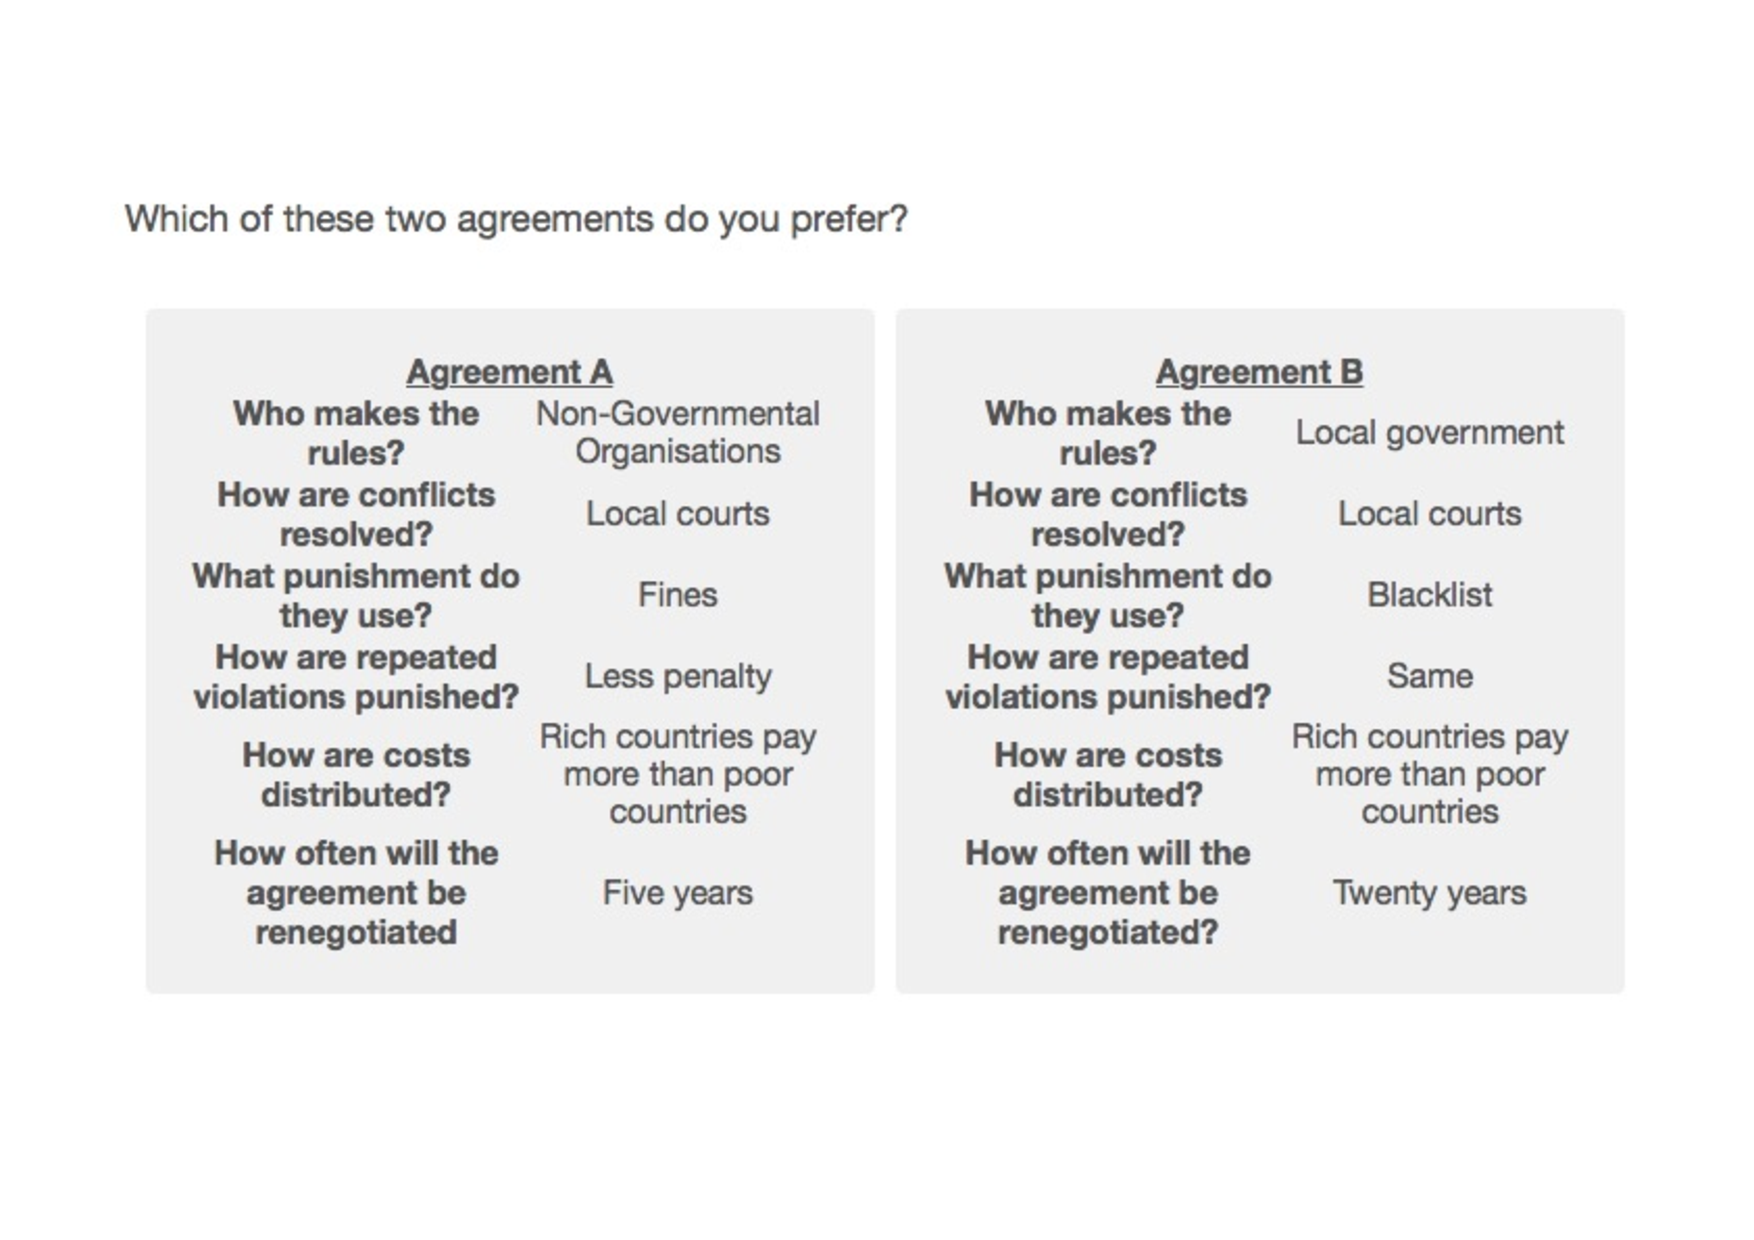
\includegraphics[width=13cm]{conjoint-cropped.pdf}
	\caption{\textbf{Example of conjoint table presented to respondents}}
	\label{fig:conjoint}
\end{figure}

We estimate our models with the \texttt{cregg} package \citep{leeper2018cregg} for the \texttt{R} statistical language \citep{rstats2019}. Here we report marginal means instead of average marginal conditional effects (AMCE) of climate agreement attributes. \citet{leeper2018subgroup} show that AMCEs can be misleading in subgroup analysis as model results are sensitive to the choice of reference categories in interactions. In contrast, marginal means provide a clear description of quantities of interest, in our case preferences towards agreement attributes, while allowing for easy comparisons between groups of respondents. Their interpretation is also straightforward: a 50\% marginal means estimate represents that respondents are indifferent when this attribute appear vis-\`{a}-vis other attributes. When the coefficient is lower than 50\%, respondents dislike packages with this attribute. Conversely, when the point estimate is higher than 50\%, respondents prefer packages containing a given attribute. Readers can refer to the Supplementary Material for AMCE estimates.

\section{Results}%
\label{sec:results}

Figure~\ref{fig:pooled} shows our main results. The graph illustrates the preference associated with each attribute of hypothetical climate mitigation agreements. Dots with horizontal bars represent point estimates and 95\% confidence intervals from linear regressions with robust standard errors clustered at the respondent level. \\

\begin{figure}[H]
	\centering
	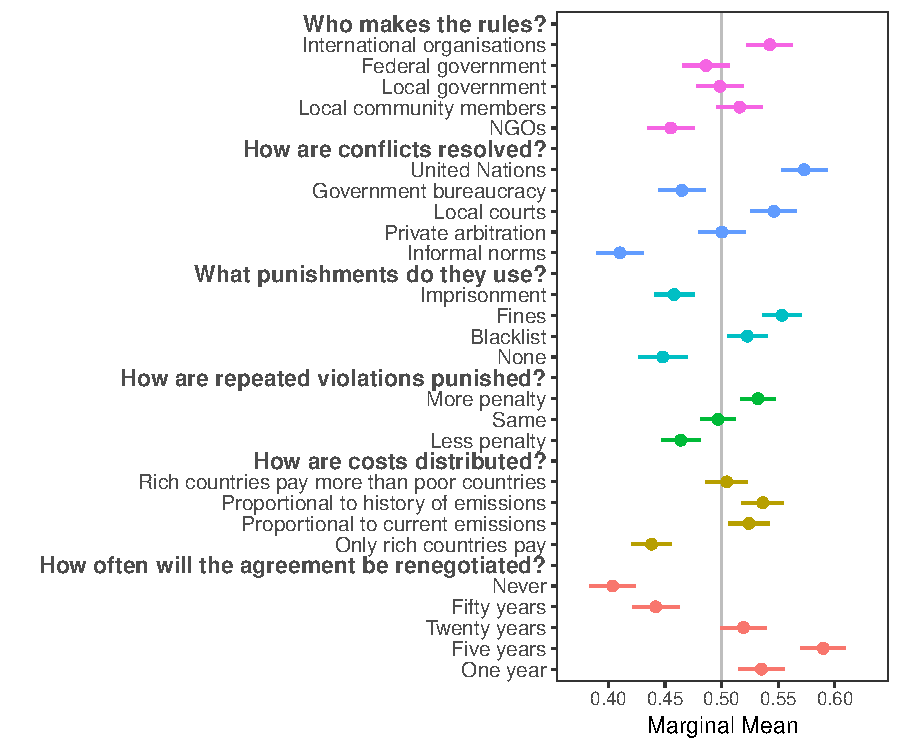
\includegraphics[width=.9\linewidth,height=11.5cm]{pooled.pdf}
	\caption{\textbf{Effect of institutional attributes on the probability of support for climate change agreements in 10 Latin American countries (pooled data)}}
	\label{fig:pooled}
\end{figure}

Respondents prefer international organisations to establish climate mitigation rules (54\%, SE = 1.2), but they also hold favourable views of local communities (51.6\%, SE = 1.25). We note that Latin American elites support multiple governance levels simultaneously, which suggests that they are willing to include separate political spheres into a single climate policy design.  Local governments (49.8\%, SE = 1.2) and state governments (48.6\%, SE = 1.3) receive slightly more support than the other alternatives, yet the difference between them is not statistically significant. Non-governmental organisations are the least preferred option for climate change rule-making with 45.5\% (SE = 1.3). 

We see a similar pattern with respect to conflict resolution. Respondents affirm disputes should be addressed mainly by the United Nations and local courts. These two choices have 57.3\% (SE = 1.2) and 54.6\% (SE = 1.2) approval, respectively. Private arbitration comes next with 50\% (SE = 1.3). Government bureaucracy and informal norms lower the chance of selecting a climate agreement, with 46.4\% (SE = 1.3) and 41\% (SE = 1.3) of support, respectively. 

Participants agree with graduated sanctions to repeated offenders (53.2\%, SE = 0.9) and they believe agreement costs should be allocated according to the country's history of emissions (53.6\%, SE = 1.1). Moreover, related to the same idea of proportionality, respondents indicate that lawbreakers should be punished with fines (55.3\%, SE = 1.1), which can be easily increased if necessary. This is in line with the literature arguing that climate change agreements present a middle ground between rigidity and flexibility to accommodate domestic demands and increase national compliance \citep{von2008international}.

Elites believe that Latin American countries should contribute to the provision of global public goods. We find no evidence that respondents intend to free ride on climate agreements, as they position themselves against the idea that rich nations should bear the costs of climate protection. This is conductive to long-term cooperation as placing the burden exclusively on rich countries is off the equilibrium path and would, presumably, not lead to a stable arrangement. 

Regarding agreement duration, respondents are interested in a balance between stability and flexibility. Interviewees reject agreements that either cannot be modified or that last for 50 years. Their preference lies in agreements that can be renegotiated every five years (59\%, SE = 1.2). This is consistent with a concern that agreements should be durable enough to provide long-term incentives to the parties, yet remain adaptable to unforeseen demands.

Overall, the results do not conform to strictly top-down or bottom-up approaches, but to a combination of these attributes. While elites favour solutions provided at the macro level, they are also open to input from other government actors and local groups. Further, the rejection on non-governmental organisations points to a discredit of self-governing arrangements as a means to deal with global warming. This result is in line with Latin America's long reliance on the state to design and implement policies.

We also examine how our results vary across countries and types of elites. Figure~\ref{fig:countries} displays the preferred climate change agreement characteristics for each of the 10 countries in our sample. The disaggregated data confirm that elites have a generalised preference for international agencies to solve conflicts, and they dislike informal norms. In addition, the cross-country results show a preference for a positive role by federal and local governments, and that local community members should also participate in the deliberation process.

\begin{figure}[H]
	\centering
	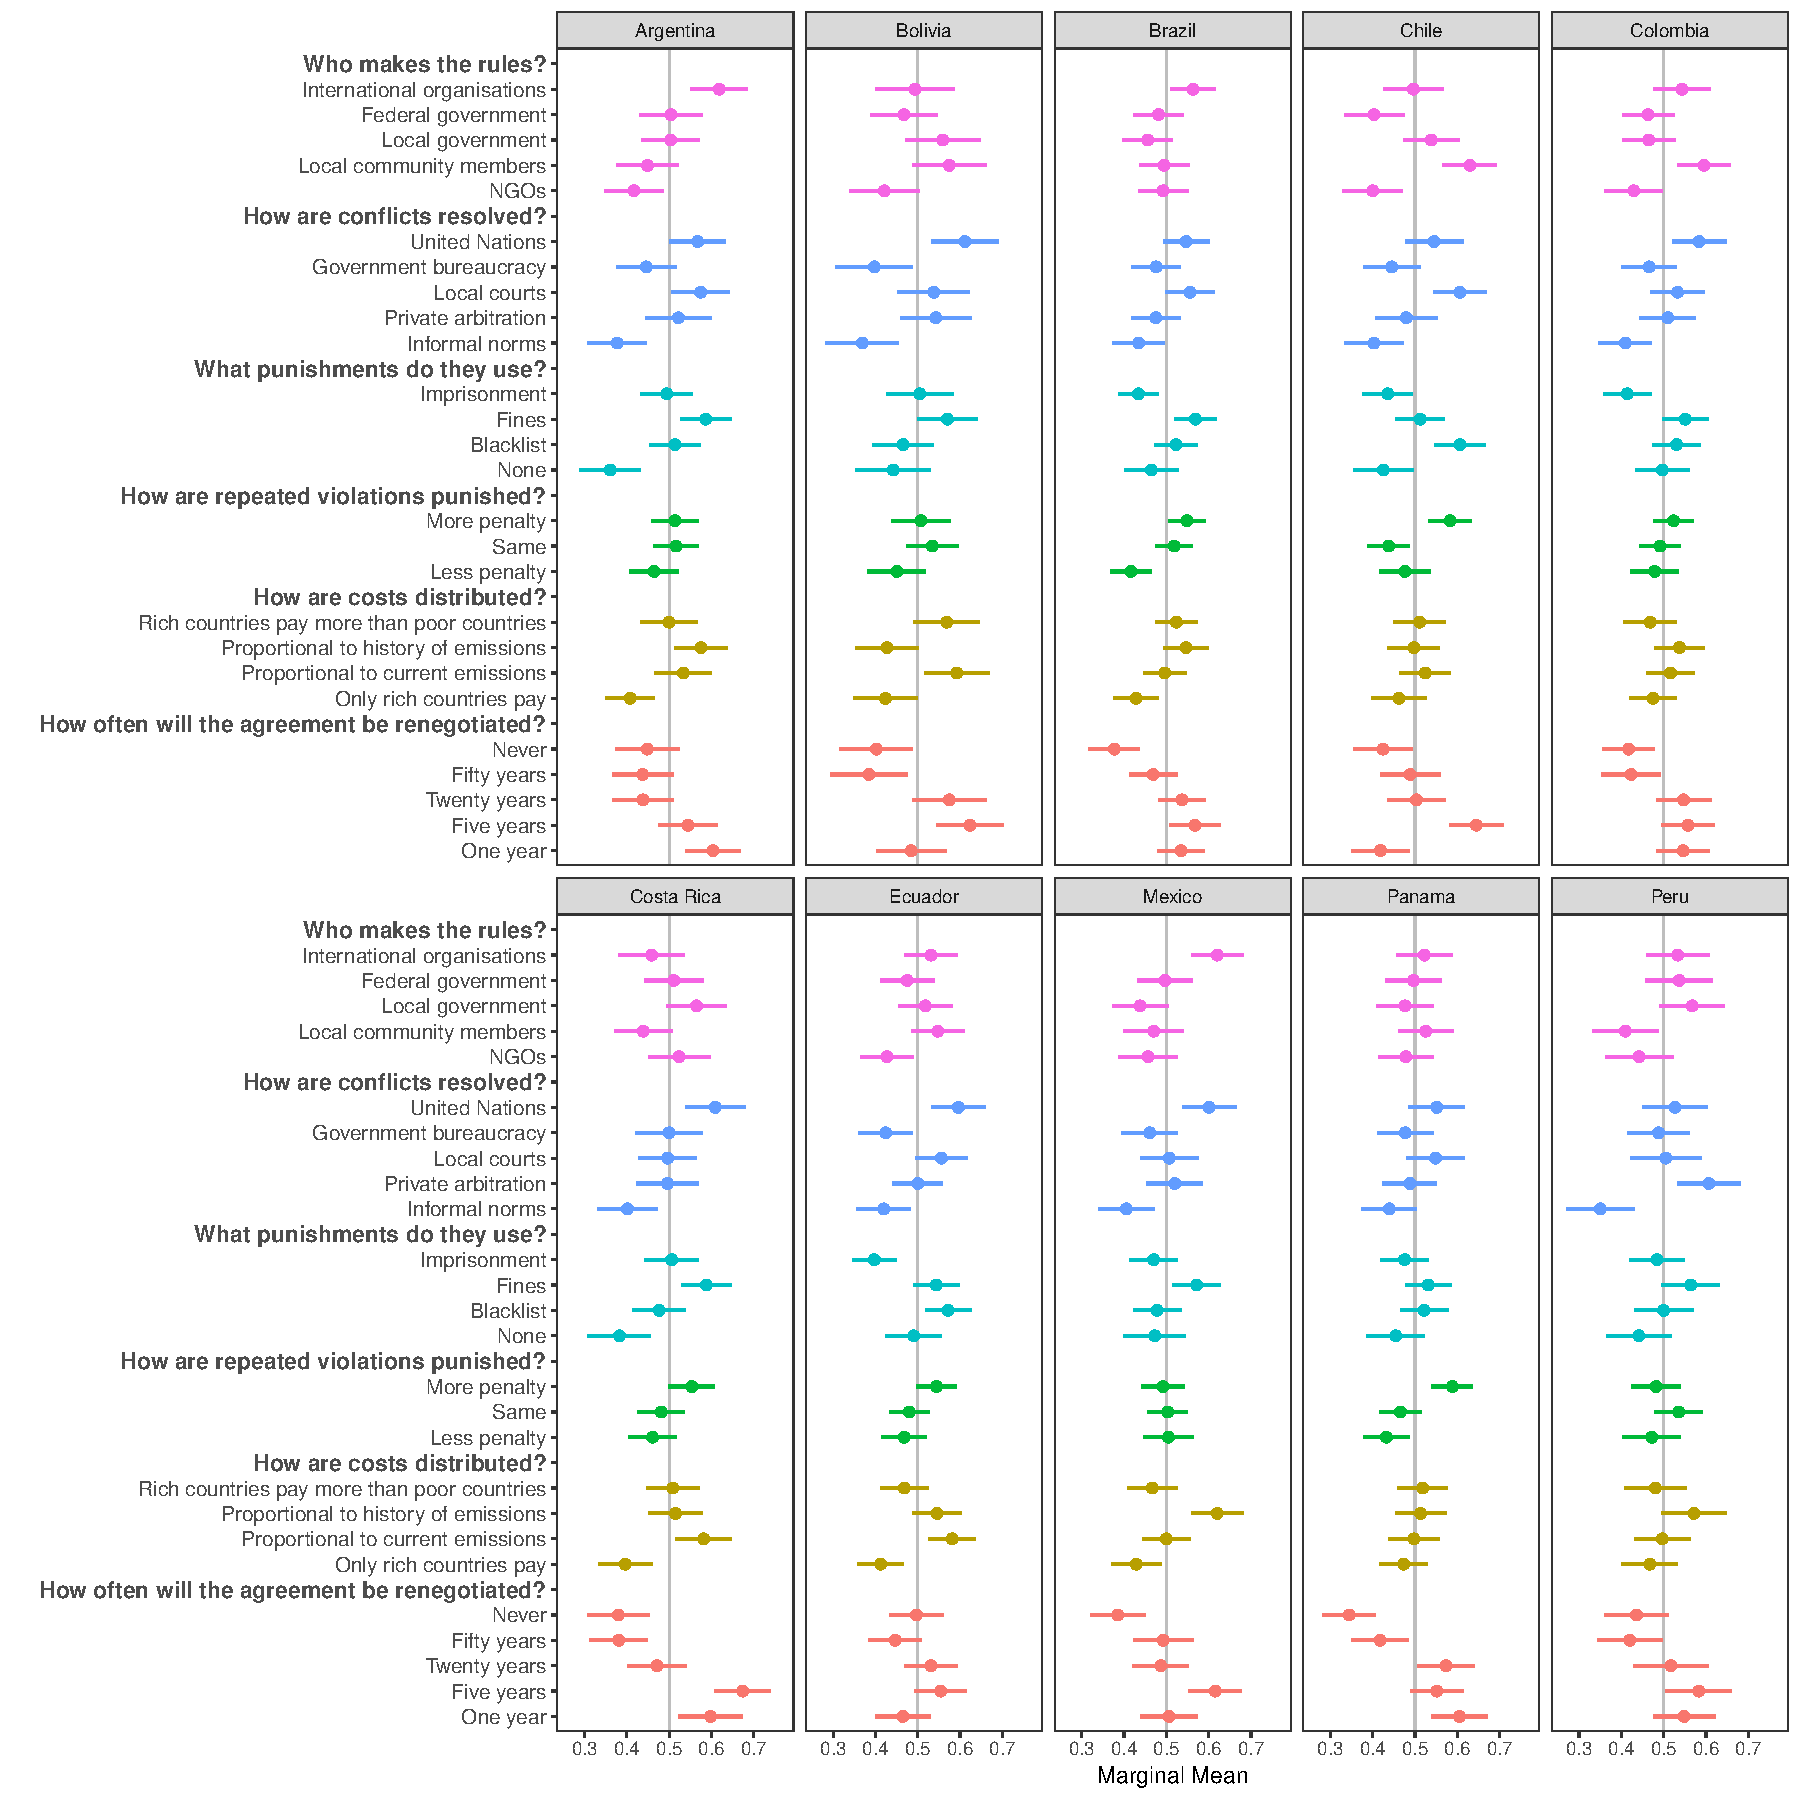
\includegraphics[width=\linewidth]{countries.pdf}
	\caption{\textbf{Effect of institutional attributes on the probability of support for climate change agreement by country}}
	\label{fig:countries}
\end{figure}

However, some of the regional preferences are a by-product of sample aggregation. Latin American elites do not have a consensus on which organisations should provide the rules. For example, elites in Costa Rica prefer local to global rule-making; in Mexico, they prefer global and dislike local, similar to Peru, Argentina and Brazil; in Colombia, elites favour global and local rule-making simultaneously; and in Bolivia, respondents prefer local organisations to design climate treaties. This is an important point and has far-reaching consequences for policy design in the region. The lack of coordination on rule-making responsibilities can make decisions to cycle, lowering the chance of a Condorcet winner. Nevertheless, these dissensions can be resolved by decentralisation, boosting the idea that flexible regime complexes, such as polycentric governance schemes, may provide a solution to potential gridlocks.

Figure~\ref{fig:types} shows the results disaggregated by elite type. Academics, members of the civil society and representatives in the executive and legislative branches hold similar views about how conflicts should be resolved, what punishment to apply to lawbreakers (fines and blacklisting) and the duration of the agreements.  

\begin{figure}[H]
	\centering
	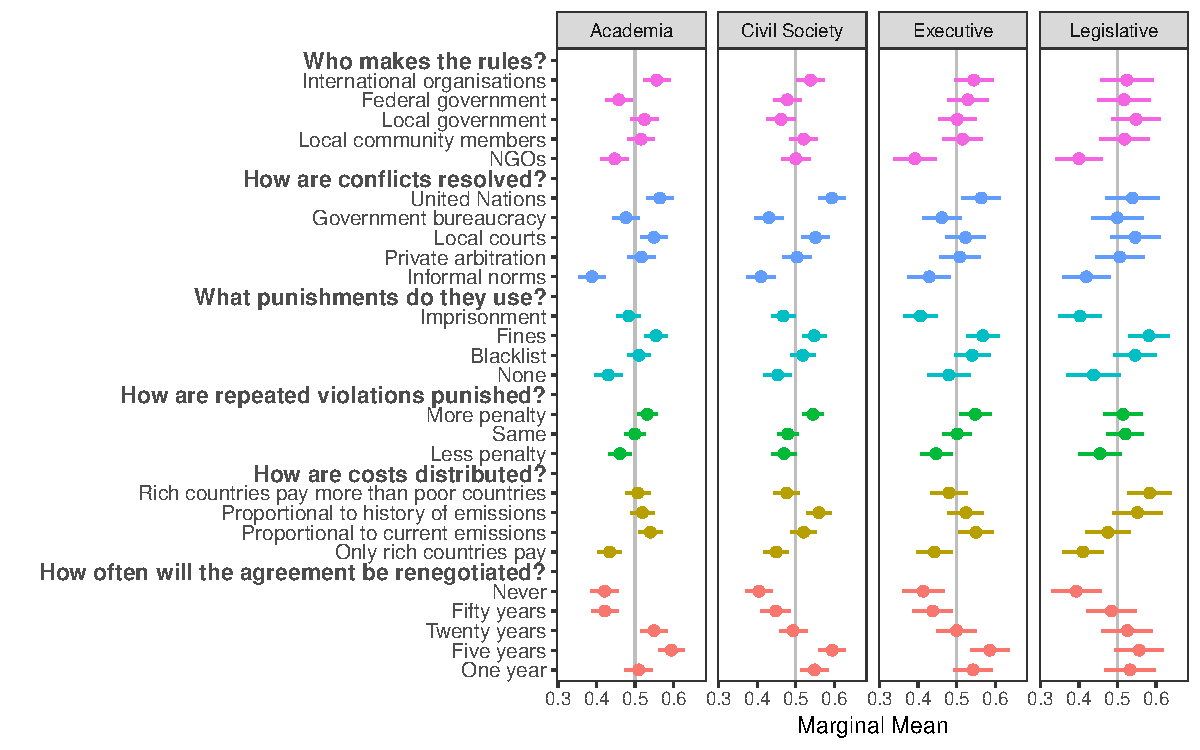
\includegraphics[width=\linewidth]{types.pdf}
	\caption{\textbf{Effect of institutional attributes on the probability of support for climate change agreement by elite type}}
	\label{fig:types}
\end{figure}

Differences emerge in two of the six attributes. Academics and members of the civil society are sceptical about the role of federal government in climate policy-making, while members of the executive and legislative -- part of the government themselves -- have a more positive view of national institutions. The differences, however, are not large. Second, members of the legislative prefer rich countries to bear the larger part of agreement costs (58.4\%, SE = 3.5). This provides evidence for the idea of historical responsibility for climate protection, an argument which developing countries have recently brought to climate negotiations \citep{muller2009differentiating,friman2015agreement}. 

\section{Discussion}%
\label{sec:discussion}

In this article, we examine which attributes of climate change mitigation treaties Latin American elites support. We find that interviewees prefer international organisations to resolve conflicts, are favourable to imposing increasing fines on violators and renewing agreements every five years. Survey participants are sceptical about non-governmental organisations and consistently reject informal norms as an instrument to solve disputes. Taken together, our evidence suggests that Latin American elites oppose non-governmental organisations as rule-makers and want legal punishment to agreement violators. 

While our results confirm that Latin Americans prefer the state to conduct public policy, they do not match the typical dichotomy of hierarchical versus decentralised climate change regimes. After disaggregating the data by country and elite type, we confirm that elites prefer international organisations to resolve disputes and that federal and local sources of governance should have a say in climate agreements. However, we find large heterogeneity in the responses, with groups holding different opinions on how competences should be divided. 

Our results have important theoretical and practical implications. The findings we present here suggest there is considerable scope for new studies on global governance, specially in underrepresented regions. Our analysis can be extended to examine if the Latin American public has the same opinion on multilevel arrangements as do the elites; and if not, it would be important to know what explains the mismatch between groups \citep{luna2005political}. Moreover, future work may address whether elites in other regions also understand climate policy as a regime complex, in which different actors play a constructive yet decentralised role in policy-making. 

With regards to environmental policies, we identify that Latin American elites are interested in incorporating different political actors and in strengthening the role of international organisations in climate governance. Building on these insights, our study provides novel information to policy-makers, as it evaluates which climate agreements are politically acceptable to Latin American elites. Future climate negotiations can achieve better results if they take those preferences into account.

\section*{Supplementary Material}
\label{sec:supplementary}

The data, code and any additional materials required to replicate all analyses in this article are available at \href{http://github.com/danilofreire/climate-governance}{\texttt{http://github.com/danilofreire/climate-governance}}.

\bibliographystyle{apalike}
\bibliography{references.bib}

\end{document}
